\documentclass[12pt]{exam}

\usepackage[margin=0.5in]{geometry}
\usepackage{amsmath,amssymb}
\usepackage{tikz,soul}
\usepackage{diagbox}
\usetikzlibrary{arrows,automata,positioning}

\newcommand{\ds}{\displaystyle}
\newcommand{\bs}{\backslash}
\newcommand{\on}{\operatorname}
\newcommand{\R}{\mathbb{R}}
\newcommand{\Z}{\mathbb{Z}}
\newcommand{\N}{\mathbb{N}}

\begin{document}
\pagestyle{empty}
\subsubsection*{Homework 4 - Computer Science 461 \hfill Name: \underline{\hspace*{2in}}}

\textit{Due Monday, Feb 10.} % You can e-mail your code for the computer programming problems to me at }\verb|blins@hsc.edu|.

\begin{questions}

\question Convert the following NFA to a DFA. Use the method we discussed in class, where the states of the DFA correspond to subsets of the states of the original NFA.  Hint: \textit{After removing states in the DFA that you can never reach, you should only need a small number of states, one of which corresponds to the empty set.}
\begin{flushright}
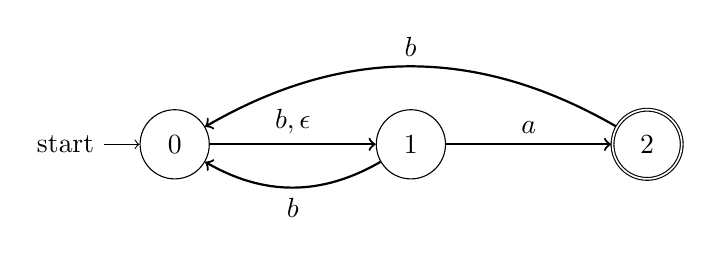
\begin{tikzpicture}[node distance=3cm,auto]
  %\tikzstyle{every state}=[fill={rgb:black,1;white,10}]

  \node[state,initial]   (q_0)                {$0$};
  \node[state]           (q_1) [right of=q_0] {$1$};
  \node[state,accepting]                     (q_2) [right of=q_1] {$2$};
  \path[thick,->]
  (q_0) edge              node {$b,\epsilon$} (q_1)
  (q_1) edge              node {$a$} (q_2)
        edge [bend left]  node {$b$} (q_0)
  (q_2) edge [bend right]  node[above] {$b$} (q_0);
        %edge [loop right] node {b} (); 
\end{tikzpicture}
\end{flushright}
\vfill

\question Let $\Sigma = \{0,1\}$.  Write a one-sentence description the languages defined by the following regular expressions.  For example: $\Sigma^*1$ would be any binary string that ends with a 1. 
\begin{parts}
\item $(\Sigma \Sigma)^*$. 
\vfill

\item $\Sigma^*01\Sigma^*$. 
\vfill

\item $(0\Sigma^*0)|(1\Sigma^*1)$.
\vfill

\item $(00|01|11)^*$.
\vfill
\end{parts}



\newpage
\question Find a regular expression that matches each of the following languages. In all cases, the alphabet is $\Sigma = \{0,1\}$.  
\begin{parts}
\part $\{w \in \Sigma^* : w \text{ contains at least three 1's.}\}$ 
\vfill

\part $\{w \in \Sigma^* : w \text{ contains at least two 1's and exactly one 0.}\}$
\vfill
\end{parts}


\question Let $\Sigma$ be the regular English alphabet $\{a,b,c,\ldots,z\}$.  Write a regular expression that matches all strings that contain at least two vowels (i.e., $a$,$e$,$i$,$o$,$u$).  

\vfill

\question Prove that if $L \subset \Sigma^*$ is a regular language, then the complement $\Sigma^* \backslash L$ is also a regular language. Hint: \textit{If there is a DFA $M = (Q, \Sigma, \delta, q, F)$ that recognizes $L$, describe a different DFA that recognizes the complement.}  
\vfill

%\question Let $L = \{w \in \Sigma^* : \text{ the length of }w\text{ is a power of 2} \}$. Use the pumping lemma to prove that $L$ is not a regular language.  
%
%\vfill
%
%\begin{minipage}{0.46\textwidth}
%\small
%\begin{parts}
%\part What are the sets $Q$, $\Sigma$, and $F$ in the formal description $(Q,\Sigma,\delta,q,F)$ of this machine?
%\vspace*{1in}
%
%\part What sequence of states does the machine go through on the input \verb|aabbaa|?  Does the machine accept \verb|aabbaa|? 
%\vspace*{0.8in}
%\end{parts}
%\end{minipage}
%\hfill
%%second column (no space between first and second column!)
%\begin{minipage}{0.4\textwidth}
%\begin{tikzpicture}[node distance=3cm,auto]
%  %\tikzstyle{every state}=[fill={rgb:black,1;white,10}]
%
%  \node[state,initial,accepting] (q_0)        {$q_0$};
%  \node[state]           (q_1) [right of=q_0] {$q_1$};
%  \node[state]           (q_2) [below of=q_0] {$q_2$};
%  \node[state,accepting] (q_3) [right of=q_2] {$q_3$};
%  \path[thick,->]
%  (q_0) edge [bend left] node {b} (q_1)
%        edge [loop above]  node {a} ()
%  (q_1) edge [bend left] node {b} (q_3)
%        edge [bend left] node {a} (q_2)
%  (q_2) edge [bend left] node {a} (q_1)
%        edge [bend left] node {b} (q_0)
%  (q_3) edge [bend left] node {a} (q_2)
%        edge [loop right] node {b} ();
%\end{tikzpicture}
%\vspace*{1.0in}
%\end{minipage}
%
%
%\question Design a DFA that outputs 1 if and only if the input length is divisible by 3. Draw a state diagram for you answer.
%\vfill
%\vfill
%
%\question Design a DFA that outputs 1 if and only if the input begins with 01 and ends with 01.  Draw a state diagram for your answer. 
%\vfill
%\vfill
%
%\newpage
%\question Construct an NFA with three states that accepts a string in $\{0,1\}^*$ iff it ends in 00.  
%\vfill
%\vfill
%
%\question Find a DFA that is equivalent to the NFA shown below. 
%\begin{flushright}
%\begin{tikzpicture}[node distance=3cm,auto]
%  %\tikzstyle{every state}=[fill={rgb:black,1;white,10}]
%
%  \node[state,initial,accepting] (q_0)        {$0$};
%  \node[state]           (q_1) [right of=q_0] {$1$};
%  \path[thick,->]
%  (q_0) edge [bend left] node {0,1} (q_1)
%        edge [loop above]  node {0} ()
%  (q_1) edge [bend left] node {1} (q_0);
%\end{tikzpicture}
%\end{flushright}
%\vfill
%
%\question Consider a DFA with states $Q = \{0,1,2\}$, alphabet $\Sigma = \{0,1\}$, initial state $q_0 = 0$, and accepting states $F = \{0, 1\}$.  The transition function is shown in the table below. Write a computer program that takes a string in $\Sigma^*$ as input and prints each state the DFA enters as it goes through the input string. Your program should also return 1 if the DFA accepts the string, otherwise return 0.  %Test your program on the string 1100111000.
%
%\begin{flushright}
%\begin{tabular}{c|cc} 
%\backslashbox{q}{$\sigma$} & 0 & 1 \\ \hline
%0 & 1 & 1 \\ 1 & 0 & 2 \\
%2 & 0 & 0
%\end{tabular}
%\end{flushright}
%\vfill

\end{questions}
\end{document}
